%% ========== ONLY FOR STANDALONE USE ==========
% \documentclass{standalone}

\usepackage{fontspec}
\defaultfontfeatures{Ligatures=TeX}  % -- becomes en-dash etc.
\setmonofont{Fira Mono}[Scale=MatchLowercase]

\usepackage{tikz}
\usetikzlibrary{calc,patterns,quotes,tikzmark,angles,decorations.pathreplacing}
\tikzset{fontscale/.style = {font=\relsize{#1}}}
\usepackage{feynman-tikz}

% math
\usepackage{amsmath}
\usepackage{amssymb}
\usepackage{mathtools}
\usepackage{xfrac}


\usepackage[
  mathrm=sym,        % use math font for mathrm, not text font
  math-style=ISO,
  bold-style=ISO,
  sans-style=italic,
  nabla=upright,
  partial=upright,
  warnings-off={
    mathtools-colon,
    mathtools-overbracket,
  },
]{unicode-math}

\usepackage[
  separate-uncertainty=true,
  per-mode=symbol-or-fraction,
]{siunitx}
\sisetup{math-micro=\text{µ},text-micro=µ}


% new commands
\newcommand{\code}[2]{%
  \texttt{\textcolor{#1}{\detokenize{#2}}}%
}

\usepackage{xcolor}

% define your colors here
\xdefinecolor{bioblue}{HTML}{4c5b75}
\xdefinecolor{bredongreen}{HTML}{619645}
\xdefinecolor{honeywax}{HTML}{f9a825}
\xdefinecolor{protonred}{HTML}{a12b2b}
\xdefinecolor{electronblue}{HTML}{0099d1}
\xdefinecolor{gammagreen}{HTML}{0a9e74}

\xdefinecolor{tugreen}{RGB}{132, 184, 25}
\xdefinecolor{tulightgreen}{HTML}{99b560}
\xdefinecolor{darkmode}{HTML}{3a3d41}
\colorlet{tulight}{tugreen!20!white}
\colorlet{tudark}{tugreen!80!black}

\xdefinecolor{tuorange}{RGB}{227, 105, 19}
\xdefinecolor{tuyellow}{RGB}{242, 189, 0}
\xdefinecolor{tucitron}{RGB}{249, 219, 0}

\xdefinecolor{tublue}{RGB}{25, 132, 184}
\colorlet{tublight}{tublue!20!white}
\colorlet{tubdark}{tublue!60!black}

\xdefinecolor{yamlblue}{HTML}{a094f2}
\xdefinecolor{yamlgreen}{HTML}{00b300}
\xdefinecolor{yamlorange}{HTML}{d67c58}
\xdefinecolor{yamlpink}{HTML}{ff00ff}
\xdefinecolor{yamlyellow}{HTML}{ffd800}

\colorlet{lightgray}{darkgray!70!white}
\colorlet{lightergray}{darkgray!50!white}
% \usepackage{pagecolor}

% \setmainfont{Fira Sans}
%% ==============================================

% colours
\xdefinecolor{darkmode}{HTML}{3a3d41}
\xdefinecolor{cherenkov_blue}{HTML}{4066a3}
\colorlet{maincolour}{darkgray}
\xdefinecolor{warmyellow}{HTML}{ffbf00} % ffb300

\tikzfading[name=fade30,
  left color=transparent!0, right color=transparent!95, shading angle=30]

\tikzfading[name=fadeEAS,
  left color=transparent!0, right color=transparent!75, shading angle=30]


\begin{tikzpicture}
  \clip (-6,0) rectangle (13,9);

  % \foreach \x in {0,1,...,9}
  %   \foreach \y in {0,1,...,9}
  %     \draw[] (\x,\y) rectangle (\x+1,\y+1);

  \pgfmathsetmacro{\y}{-0.15}
  \pgfmathsetmacro{\x}{0.15}
  \pgfmathsetmacro{\globalshift}{2.5cm}

  % MOUNTAIN RANGE
  \uncover<1->{
  \path[draw=maincolour,line width=0.077pt,xshift=-0.26cm,yshift=8.6cm] (\x*-3.5061,\y*40.4408) .. controls (\x*-1.9421,\y*40.5830) and (\x*-2.3686,\y*40.6304) .. (\x*-1.7999,\y*40.5830) .. controls (\x*-1.2312,\y*40.5356) and (\x*0.9964,\y*40.8200) .. (\x*0.9964,\y*40.8200) .. controls (\x*0.9964,\y*40.8200) and (\x*1.9917,\y*41.0095) .. (\x*2.1813,\y*41.0569) .. controls (\x*2.3709,\y*41.1043) and (\x*3.9823,\y*41.2465) .. (\x*3.9823,\y*41.2465) -- (\x*5.4042,\y*41.7205) -- (\x*5.9729,\y*42.4788) -- (\x*6.9208,\y*42.7158) -- (\x*7.9635,\y*43.1423) -- (\x*8.6270,\y*43.5689) .. controls (\x*8.6270,\y*43.5689) and (\x*8.9588,\y*44.2324) .. (\x*9.1958,\y*44.3746) .. controls (\x*9.4328,\y*44.5168) and (\x*10.1911,\y*44.6116) .. (\x*10.3807,\y*44.7064) .. controls (\x*10.5702,\y*44.8012) and (\x*11.1390,\y*44.8959) .. (\x*11.3286,\y*44.9433) .. controls (\x*11.5182,\y*44.9907) and (\x*11.7551,\y*45.1329) .. (\x*11.9921,\y*45.4173) .. controls (\x*12.2291,\y*45.7017) and (\x*12.9400,\y*46.0334) .. (\x*13.1296,\y*46.0808) .. controls (\x*13.3192,\y*46.1282) and (\x*14.3145,\y*46.4600) .. (\x*14.5514,\y*46.5548) .. controls (\x*14.7884,\y*46.6496) and (\x*16.1629,\y*46.8391) .. (\x*16.4473,\y*46.8391) .. controls (\x*16.7316,\y*46.8391) and (\x*17.9165,\y*46.6970) .. (\x*17.9165,\y*46.6970) .. controls (\x*17.9165,\y*46.6970) and (\x*18.5800,\y*46.7918) .. (\x*18.8644,\y*46.8391) .. controls (\x*19.1488,\y*46.8865) and (\x*20.1915,\y*46.6970) .. (\x*20.1915,\y*46.6970) .. controls (\x*20.1915,\y*46.6970) and (\x*20.8076,\y*46.1282) .. (\x*21.2342,\y*46.2704) .. controls (\x*21.6607,\y*46.4126) and (\x*23.6039,\y*46.6496) .. (\x*23.6039,\y*46.6496) -- (\x*24.7414,\y*46.4600) -- (\x*25.8789,\y*46.1756) .. controls (\x*25.8789,\y*46.1756) and (\x*26.5898,\y*46.2230) .. (\x*26.7794,\y*46.2230) .. controls (\x*26.9690,\y*46.2230) and (\x*29.2440,\y*46.1282) .. (\x*29.2440,\y*46.1282) .. controls (\x*29.2440,\y*46.1282) and (\x*30.7132,\y*45.7017) .. (\x*30.9028,\y*45.7017) .. controls (\x*31.0924,\y*45.7017) and (\x*32.4194,\y*45.4173) .. (\x*32.4194,\y*45.4173) -- (\x*33.9835,\y*45.2277) -- (\x*35.4527,\y*45.0381) .. controls (\x*35.4527,\y*45.0381) and (\x*37.4907,\y*44.7064) .. (\x*37.6803,\y*44.7064) .. controls (\x*37.8699,\y*44.7064) and (\x*39.2917,\y*44.4220) .. (\x*39.4813,\y*44.4220) .. controls (\x*39.6709,\y*44.4220) and (\x*41.6141,\y*44.2798) .. (\x*41.6141,\y*44.2798) .. controls (\x*41.6141,\y*44.2798) and (\x*42.3250,\y*43.9006) .. (\x*42.5620,\y*43.9006) .. controls (\x*42.7990,\y*43.9006) and (\x*45.2635,\y*43.6637) .. (\x*45.2635,\y*43.6637) .. controls (\x*45.2635,\y*43.6637) and (\x*46.2588,\y*43.5689) .. (\x*46.4958,\y*43.5215) .. controls (\x*46.7328,\y*43.4741) and (\x*46.9224,\y*43.4267) .. (\x*47.6333,\y*43.4267) .. controls (\x*48.3442,\y*43.4267) and (\x*50.0978,\y*43.2845) .. (\x*50.0978,\y*43.2845) -- (\x*51.4723,\y*42.9053) .. controls (\x*51.4723,\y*42.9053) and (\x*51.8989,\y*42.7158) .. (\x*52.3254,\y*42.7158) .. controls (\x*52.7520,\y*42.7158) and (\x*53.9843,\y*42.5736) .. (\x*54.3160,\y*42.5262) .. controls (\x*54.6478,\y*42.4788) and (\x*55.7853,\y*42.4314) .. (\x*55.7853,\y*42.4314) .. controls (\x*55.7853,\y*42.4314) and (\x*57.0175,\y*42.5262) .. (\x*57.3019,\y*42.7158) .. controls (\x*57.5863,\y*42.9053) and (\x*59.4347,\y*43.4741) .. (\x*59.4347,\y*43.4741) -- (\x*60.1456,\y*43.7111) -- (\x*61.3068,\y*43.8533) -- (\x*62.4917,\y*43.5452) -- (\x*62.8709,\y*43.4978) -- (\x*63.5818,\y*43.4978);
  \path[draw=maincolour,line width=0.077pt,xshift=-0.26cm,yshift=8.6cm] (\x*63.5708,\y*43.4981) -- (\x*65.2770,\y*43.2137) -- (\x*66.7937,\y*43.2137) -- (\x*67.9312,\y*42.9293) -- (\x*69.6374,\y*43.2137) -- (\x*70.5853,\y*43.6877) -- (\x*72.0071,\y*44.1616) -- (\x*74.5665,\y*44.3512) .. controls (\x*74.5665,\y*44.3512) and (\x*76.5571,\y*43.3085) .. (\x*76.9362,\y*43.2137) .. controls (\x*77.3154,\y*43.1189) and (\x*78.7373,\y*42.8345) .. (\x*78.7373,\y*42.8345) -- (\x*79.5904,\y*43.0241) -- (\x*81.9601,\y*44.8251) -- (\x*84.7091,\y*46.0574) -- (\x*85.5622,\y*46.7209) -- (\x*87.5528,\y*47.0053) -- (\x*88.3111,\y*46.9105) -- (\x*89.8277,\y*47.1949) -- (\x*92.4819,\y*47.7636) -- (\x*95.0412,\y*47.5741) -- (\x*97.5058,\y*48.3324) -- (\x*99.0224,\y*48.2376) -- (\x*100.0651,\y*48.2376) -- (\x*101.2026,\y*47.8584) -- (\x*103.4776,\y*47.1001) .. controls (\x*103.4776,\y*47.1001) and (\x*103.9515,\y*46.9105) .. (\x*104.3307,\y*46.9105) .. controls (\x*104.7098,\y*46.9105) and (\x*106.0369,\y*47.0053) .. (\x*106.0369,\y*47.0053) .. controls (\x*106.0369,\y*47.0053) and (\x*106.7952,\y*47.4793) .. (\x*107.1744,\y*47.4793) .. controls (\x*107.5535,\y*47.4793) and (\x*109.9233,\y*47.4793) .. (\x*109.9233,\y*47.4793) -- (\x*112.2931,\y*47.0053);
  \path[draw=maincolour,line width=0.077pt,xshift=-0.26cm,yshift=8.6cm] (\x*-3.4472,\y*40.4288) -- (\x*-4.2683,\y*40.3785) -- (\x*-5.0726,\y*40.0936) -- (\x*-5.9105,\y*40.2277) -- (\x*-6.3964,\y*40.2779);
  \path[draw=maincolour,line width=0.077pt,xshift=-0.26cm,yshift=8.6cm] (\x*-6.3671,\y*40.2780) -- (\x*-7.4228,\y*40.3115) -- (\x*-7.9422,\y*40.3617) -- (\x*-8.4449,\y*40.5628) -- (\x*-8.7130,\y*40.5628) -- (\x*-9.0649,\y*40.7136) -- (\x*-9.3833,\y*40.8644) -- (\x*-9.6011,\y*41.0152) .. controls (\x*-9.6011,\y*41.0152) and (\x*-9.7855,\y*41.1493) .. (\x*-9.8525,\y*41.1661) .. controls (\x*-9.9195,\y*41.1828) and (\x*-10.2044,\y*41.2834) .. (\x*-10.2044,\y*41.2834) -- (\x*-10.7071,\y*41.3839) -- (\x*-11.1428,\y*41.6017) .. controls (\x*-11.1428,\y*41.6017) and (\x*-11.2098,\y*41.6352) .. (\x*-11.3438,\y*41.7358) .. controls (\x*-11.4779,\y*41.8363) and (\x*-11.7292,\y*42.0039) .. (\x*-11.8130,\y*42.0877) .. controls (\x*-11.8968,\y*42.1715) and (\x*-12.3325,\y*42.5569) .. (\x*-12.3325,\y*42.5569) -- (\x*-12.8520,\y*42.8752) -- (\x*-14.7622,\y*44.0985) -- (\x*-15.7006,\y*44.0985) -- (\x*-17.0411,\y*44.9698) -- (\x*-17.7114,\y*45.1709) -- (\x*-18.1806,\y*45.1709) -- (\x*-18.9179,\y*45.3050) -- (\x*-19.9903,\y*45.7071) -- (\x*-21.5319,\y*45.5731) -- (\x*-22.3363,\y*45.6401) -- (\x*-23.4757,\y*45.5731) -- (\x*-25.1514,\y*45.5061) -- (\x*-26.2909,\y*45.5731) -- (\x*-27.3633,\y*45.7742) -- (\x*-29.3071,\y*46.7796) -- (\x*-30.5135,\y*47.1147) -- (\x*-31.3179,\y*47.0477) .. controls (\x*-31.3179,\y*47.0477) and (\x*-32.2562,\y*46.6455) .. (\x*-32.5244,\y*46.5785) .. controls (\x*-32.7925,\y*46.5115) and (\x*-33.5298,\y*46.3104) .. (\x*-33.5298,\y*46.3104) -- (\x*-35.1384,\y*45.5731) -- (\x*-36.3449,\y*44.7017) -- (\x*-37.6184,\y*44.3666) -- (\x*-38.5568,\y*44.3666) -- (\x*-39.9643,\y*43.1601) .. controls (\x*-39.9643,\y*43.1601) and (\x*-40.9698,\y*42.7579) .. (\x*-41.3719,\y*42.5569) .. controls (\x*-41.7741,\y*42.3558) and (\x*-43.0476,\y*42.1547) .. (\x*-43.0476,\y*42.1547) -- (\x*-45.7957,\y*42.7579) -- (\x*-47.0022,\y*43.4282) -- (\x*-48.1416,\y*43.1601) .. controls (\x*-48.1416,\y*43.1601) and (\x*-48.8119,\y*42.6909) .. (\x*-49.1470,\y*42.6239) .. controls (\x*-49.4822,\y*42.5569) and (\x*-50.6216,\y*42.7579) .. (\x*-50.6216,\y*42.7579) -- (\x*-52.2303,\y*42.2888) -- (\x*-53.7049,\y*42.6909) .. controls (\x*-53.7049,\y*42.6909) and (\x*-54.0400,\y*43.1601) .. (\x*-54.4422,\y*43.1601) .. controls (\x*-54.8443,\y*43.1601) and (\x*-55.2465,\y*43.2271) .. (\x*-55.5146,\y*43.3612) .. controls (\x*-55.7827,\y*43.4952) and (\x*-56.4530,\y*43.8974) .. (\x*-56.4530,\y*43.8974) .. controls (\x*-56.4530,\y*43.8974) and (\x*-56.7211,\y*44.0985) .. (\x*-57.0562,\y*44.4336) .. controls (\x*-57.3914,\y*44.7688) and (\x*-57.3914,\y*44.8358) .. (\x*-57.7265,\y*45.1039) .. controls (\x*-58.0616,\y*45.3720) and (\x*-59.0670,\y*45.9752) .. (\x*-59.0670,\y*45.9752) -- (\x*-59.6703,\y*46.4444) -- (\x*-61.6140,\y*47.3158) -- (\x*-62.9546,\y*47.8520) -- (\x*-63.5578,\y*47.7850) -- (\x*-65.4346,\y*48.1871) -- (\x*-67.4454,\y*47.5169) -- (\x*-69.8584,\y*48.1871) -- (\x*-72.2713,\y*48.3212) -- (\x*-74.4162,\y*48.8574) -- (\x*-77.3654,\y*48.9915);

  \draw[maincolour!40!white] (-7, 1) -- (14, 1);
  }

  \node[xshift=\globalshift+1cm] at (8,2.3) {\reflectbox{\includegraphics[height=0.4cm]{build/tikz/xkcd_light.pdf}}};

  % CHERENKOV LIGHT POOL
  \uncover<4->{
  \fill[opacity=0.7, path fading=fade30, left color=cherenkov_blue, right color=cherenkov_blue, xshift=\globalshift] (0,8) -- (3,0) -- (9,0) -- cycle;
  }

  % CHERENKOV RADIATION
  \only<4>{
    \node [] at (-2.3, 6) {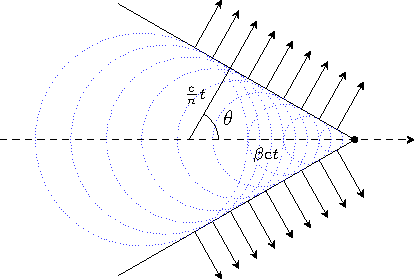
\includegraphics[height=5.7cm]{build/tikz/cherenkov_radiation.pdf}};
  }

  % INITIAL GAMMA
  \uncover<2->{
  \draw[warmyellow, xshift=\globalshift] (-0.65,9) -- (0.1,7.85) node[midway, above right, maincolour] {\large $\gamma$-ray entering the atmosphere};
  }
  % EXTENSIVE AIR SHOWER
  \uncover<3->{
  \fill[opacity=1, path fading=fadeEAS, left color=warmyellow, right color=warmyellow, xshift=\globalshift] (0,8) -- (1,6) arc(30:200:-0.35) -- cycle;
  }

  % HEITLER MODEL
  \only<3>{
    \node [] at (-2.3, 6) {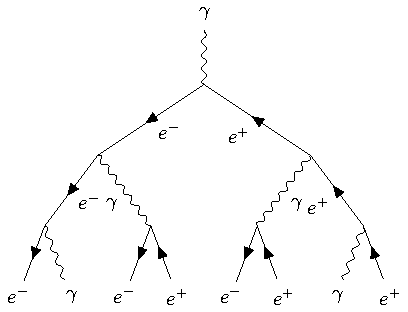
\includegraphics[height=5.7cm]{build/tikz/heitler_model.pdf}};
  }

  % TELESCOPES
  \node[inner sep=15pt, xshift=\globalshift] at (6,1.3){\reflectbox{\includegraphics[height=2.5cm]{graphics/contours_mst_dark.pdf}}};
  \node[inner sep=15pt, xshift=\globalshift] at (4,1.3){\reflectbox{\includegraphics[height=2.5cm]{graphics/contours_mst_dark.pdf}}};

  % DESCRIPTIONS
  \uncover<4->{
  \path[maincolour, every node/.style={font=\sffamily\small}, ->, >=latex, xshift=\globalshift] (5,5) edge[bend right] node [left] {} (4,4.445);
  \node[maincolour, right, xshift=\globalshift] at (5,5) {\large Pool of Cherenkov light};
  }
  \uncover<3->{
  \path[maincolour, every node/.style={font=\sffamily\small}, ->, >=latex, xshift=\globalshift] (2,7) edge[bend right] node [left] {} (1.3,6.5);
  \node[maincolour, right, xshift=\globalshift] at (2,7) {\large Extensive Air Shower (EAS)};
  }

  % CAMERA FRAME
  \uncover<5->{
  \node [circle, draw, color=maincolour, fill=darkmode, minimum width = 2.5cm, path picture = {
    \node [] at (path picture bounding box.center) {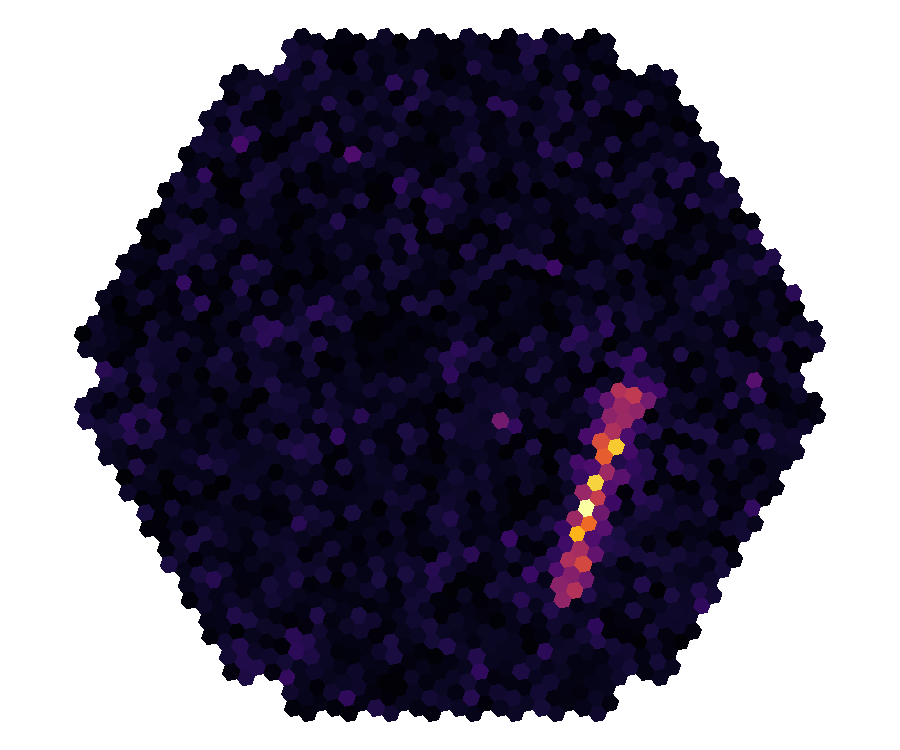
\includegraphics[height=2.8cm]{graphics/mst_camera_frame.pdf}};
    }, xshift=\globalshift] (CAMERAFRAME) at (-0.5,2) {};

  \node [above, yshift=1.3cm] at (CAMERAFRAME) {\large Snapshot in camera frame};

  \path[maincolour, every node/.style={font=\sffamily\small}, ->, >=latex, xshift=\globalshift] (3.2,2.6) edge[bend right] (CAMERAFRAME);
  }


\end{tikzpicture}
